\documentclass[pt,bsc,oneside,onehalfspacing]{risethesis}

\usepackage{natbib}
\usepackage{babel}
\usepackage{supertabular}
\usepackage{fancybox}
\usepackage{acronym}
\usepackage{moreverb}

\usepackage[linkcolor=black,citecolor=black,urlcolor=black,colorlinks,pdfpagelabels,pdftitle={srp-tcs5},pdfauthor={Tarcisio Coutinho da Silva}]{hyperref}

\renewcommand{\appendixtocname}{Apêndices} 
\renewcommand{\appendixpagename}{Apêndices}

\address{Recife}

\universitypt{Universidade Federal de Pernambuco}
\universityen{Federal University of Pernambuco}

\departmentpt{Centro de Informática}
\departmenten{Center for Informatics}

\programpt{Graduação em Ciência da Computação}
\programen{Graduate in Computer Science}

\majorfieldpt{Ciência da Computação}
\majorfielden{Computer Science}

\title{Um Mecanimos de Monitoramento de Serviços para a Manutenção de Contratos com Base em Atributos de Qualidade}
\date{dezembro/2011}

\author{Tarcisio Coutinho da Silva}
\adviser{Nelson Souto Rosa}


\begin{document}

\frontmatter
\frontpage
\presentationpage

\begin{dedicatory}
%TODO: Dedicatoria rápida
\ldots
\end{dedicatory}

\acknowledgements
%TODO: Agradecimentos
\ldots

\begin{epigraph}[Shiawase no Iro]{Yoko Ishida}
Oozora ni egaita\\
Chiisana yume wo taisetsu ni shiyou\\
Sousureba itsumo shiawase ni nareru\\
Kitto.\\
\vspace{0.5cm}
Dê importância ao pequeno sonho que você pintou em direção ao céu\\
Se fizer isto, você sempre será feliz\\
Certamente.
\vspace{0.2cm}
\end{epigraph}

% Abstract
\resumo
\paragraph{}
Arquitetura Orientada a Serviços, ou do inglês \textit{Service-Oriented Architecture} (SOA), tem surgido ao longo dos últimos anos como uma das abordagens preferidas para construção de sistemas. Com objetivos alinhados aos objetivos do paradigma SOC \textit{(Service-Oriented Computing)}, SOA possibilita a criação de novas aplicações com maior coerência, rapidez e diminuição nos custos, tudo isso com excelente aproveitamento do legado.
Deste modo, a contrução de aplicações orientadas a serviços tende a ter maior agilidade, flexibilidade e reuso de componentes pré-existentes.
Nesse contexto, módulos podem consumir serviços providos por tecnologias diferentes, apenas identificando o serviço requerido e realizando o \textit{binding}. Estabelecendo assim um contrato entre o consumidor e o provedor do serviço.
%TODO: Colocar novo objetivo

\begin{keywords}

\end{keywords}


\abstract
TODO:
\begin{keywords}

\end{keywords}



\tableofcontents
\listoffigures
\listoftables
% Lista de Siglas
\chapter*{Lista de Abreviaturas}
\addcontentsline{toc}{chapter}{Lista de Abreviaturas}
\begin{acronym}
	\acro{SOA}{Service Oriented Architecture}
	\acro{SOC}{Service Oriented Computing}
	\acro{DBC}{Desenvolvimento Baseado em Componentes}
	\acro{TI}{Tecnologia da Informaç\~ao}
	\acro{UFPE}{Federal University of Pernambuco}
	\acro{NFR}{Non-Functional Requirement}
	\acro{SLA}{Service Level Agreement}
	\acro{OSGi}{Open Services Gateway Initiative}
	\acro{JMX}{Java Management Extensions}
\end{acronym}

\mainmatter

% Capitulos
\chapter{Introdução}
\label{ch:1}

\section{Contexto}
Atualmente, o mercado cada vez mais acirrado e competitivo, faz com que as empresas constantemente modifiquem e redesenhem suas estratégias de negócio de maneira ágil, buscando incessantemente por inovação e agregação de valor a seus produtos e serviços. 

Esse tipo de cenário, do ponto de vista computacional, requer adaptação constante dos sistemas e processos relacionados, tornando os custos necessários a essa adaptação um grande obstáculo~\cite{papazoglou2008service}~\cite{rabelo2006}, já que a maioria desses custos são provenientes de implementações de novas soluções para cada caso específico. Além disso, o constante incremento de novas aplicações torna o sistema ainda mais complexo, dificultando o processo de desenvolvimento e aumentando também os custos relacionados ao gerenciamento~\cite{rabelo2006}~\cite{ada2006}.

Assim, é clara a necessidade de uma solução que suportasse esse novo contexto, no qual os sistemas constantemente evoluem, interagem e trocam informações entre si, onde a idéia de se desenvolver uma aplicação nova e complexa deve ser evitada e substituída por um conjunto de aplicações pequenas, já existentes (quando possível) e mais simples~\cite{rabelo2006}. A aplicação agora deve ser composta por um conjunto de módulos independentes, especializados, interoperáveis e sobretudo simples, o que aumenta a reutilização e manutenção do módulo~\cite{oracle2005ws}.

Em função disto, temos nos princípios de SOA, um modelo arquitetural modular e interoperável que se mostra como uma alternativa viável à resolução dessa necessidade.

Arquitetura Orientada a Serviços, ou do inglês \textit{Service Oriented Architecture} (SOA), tem surgido ao longo dos últimos anos como uma das abordagens preferidas para construção de sistemas~\cite{erl2008soa}. Com objetivos alinhados aos objetivos do paradigma SOC \textit{(Service-Oriented Computing)}~\cite{papazoglou:2003}, SOA possibilita a criação de novas aplicações com maior coerência, rapidez e diminuição nos custos, tudo isso com excelente aproveitamento do legado~\cite{erl2008soa}.

Baseada em padrões abertos e na visão onipresente da Internet, SOA tem como princípio fundamental a idéia de serviços como unidades que representam módulos do negócio ou funcionalidades da aplicação~\cite{erl2008soa}~\cite{imb2007soa}~\cite{cervantes2005technical}. Na visão de SOA, um serviço é um componente que implementa uma função de negócio. Ele pode responder a requisições ocultando os detalhes de sua implementação e é descrito através de contratos que expressam seu objetivo e suas capacidades. 

Buscando maior agilidade, flexibilidade e reuso de componentes pré-existentes no desenvolvimento de aplicações, diversas empresas de tecnologia da informação vêm adotando SOA na construção de seus sistemas. O modelo básico de SOA, consiste em 3 elementos principais apresentados na figura \ref{fig:soatriangle}.

O \textbf{provedor do serviço} (\textit{Service Provider}), que implementa a função de negocio e publica uma descrição do serviço no registro. O \textbf{registro} (\textit{Service Registy}) que dá suporte à capacidade de descobrimento de serviços (\textit{Discoverability}), já que, provedores tem de publicar seus serviços para que estes possam ser consumidos por potenciais consumidores que realizam uma busca pelo serviço que necessitam no registro. E o \textbf{consumidor do serviço} (\textit{Service Requestor}) que busca no registro por um determinado serviço, caso este seja encontrado, a localização do serviço é recuperada e o consumidor se conecta ao endpoint do serviço, podendo assim invocar as operações do serviço~\cite{michlmayr2007towards}~\cite{huhns2005service}.

\begin{figure}[htp]
\centering
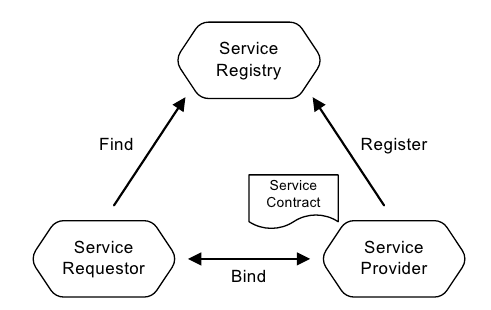
\includegraphics[width=7cm]{chapters/intro/soa_triangle.png}
\caption[Triângulo SOA]{Triângulo SOA~\cite{michlmayr2009end}.}
\label{fig:soatriangle}
\end{figure}

A figura \ref{fig:soatriangle} mostra de maneira implícita alguns dos princípios essenciais de SOC, a flexibilidade e o baixo acoplamento entre serviços, uma vez que, um provedor de serviços pode muito bem fazer o papel consumidor de serviços. Essa dinâmica tem impactos ainda maiores quando tratamos de arquitetura de software. Pois, ao trocarmos aplicações monolíticas por serviços ou composições de serviços, estes pequenos módulos podem ser facilmente substituídos ou atualizados, sem que haja um impacto maior no sistema.

Nesse contexto, temos a plataforma de serviços OSGi (\textit{Open Services Gateway initiative}~\cite{alliance2007osgi}. OSGi provê suporte à modelagem e desenvolvimento de sistemas modulares na linguagem Java~\cite{hall2010osgi}. A idéia básica é resolver o problema de criar softwares monolíticos, ou seja, softwares projetados sem modularidade, facilitando a reutilização e manutenção de  componentes, o que torna a solução mais robusta, barata e confiável~\cite{davis2009open}.

OSGi introduz um modelo de programação orientada a serviço, o que alguns autores apresentam como \textit{SOA in a Virtual Machine}~\cite{hall2010osgi}, separando de fato a interface da implementação. Isso mostra um grande potencial para a construção de aplicações orientadas à serviço.

Outra tecnologia que compartilha vários princípios de SOC é a tecnologia de \textit{Web Services}. \textit{Web Services} fornecem uma forma padrão de interoperabilidade entre diferentes aplicações, capaz de executar em uma variedade de plataformas e \textit{frameworks}~\cite{w3c2002ws} simplificando o desenvolvimento de aplicações distribuídas.

Assim, em uma arquitetura orientada a serviços, módulos podem consumir serviços providos por tecnologias diferentes, apenas identificando o serviço requerido e realizando o \textit{binding}. Estabelecendo assim um contrato entre o consumidor e o provedor do serviço~\cite{oracle2005ws}.

Esses contratos são especificados através de SLAs (\textit{Service Level Agreement}). Em um SLA temos basicamente uma descrição de um acordo entre o provedor e consumidor de um determinado serviço. Esse acordo define as responsabilidades de ambas as partes, as propriedades de como consumidor terá acesso ao serviço (geralmente relacionadas a requisitos não-funcionais, como: \textit{response time} e disponibilidade), a duração do contrato, entre outros~\cite{jin2002analysis}~\cite{slasoi}.

Porém, uma tarefa complexa neste cenário é garantir que os acordos a nível de serviço, SLAs, entre o consumidor e provedor são realmente respeitados. Além disso, prevenir uma quebra de contrato, onde o provedor não cumpre com os requisitos não-funcionais definidos nos SLAs, é outro ponto complexo a ser atacado, pois, na maioria dos casos, quando é caracterizada uma quebra de contrato o provedor pode sofrer algum tipo de penalidade, ou mesmo, perder um potencial consumidor de seus serviços.

Deste modo, o monitoramento dos serviços aliado à análise dos dados monitorados, surge como uma possível solução para o problema de garantir o cumprimento dos contratos entre provedores e consumidores de serviços~\cite{papazoglou2008service}. Ainda mais, o resultado dessa análise aliada a um mecanismo de auto-gerenciamento do ambiente onde estes serviços são executados, surge como uma alternativa viável à manutenção dos contratos por parte dos provedores. Uma vez que, na definição dos SLAs, o provedor apresenta suas capacidades funcionais e não-funcionais (atributos de QoS), e os consumidores ao buscarem serviços, definem contratos com base nessas informações disponibilizadas por esses provedores, comprovando as necessidades citadas acima.

\section{Objetivos}
\label{sec:obj}

O objetivo desse trabalho é especificar e construir, com base nas ideias do ciclo de desenvolvimento PCDA (ver Seção \ref{sec:pdca}), um mecanismo de gerenciamento automático de provedores de serviço, focado na prevenção de possíveis quebras de contrato.

A prevenção da quebra será realizada através do monitoramento de atributos de qualidade relacionados a invocações a um determinado serviço e do balanceamento de carga em função do contexto em que o serviço provido é executado. 

Assim, as ações de gerenciamento são realizadas dinamicamente (em tempo de execução), sem que o serviço provido torne-se indisponível.



\section{Organização do Trabalho}
Visando atingir o objetivo proposto na Seção \ref{sec:obj}, o trabalho foi organizado da seguinte maneira:
\begin{itemize}

\item \textbf{Capítulo 2 - Conceitos Básicos}

Neste capítulo serão apresentados os principais conceitos necessários ao entendimento do trabalho. Discutiremos sobre orientação a serviços, orientação a componentes, OSGi e iPOJO, o ciclo PCDA e gerenciamento com JMX. A apresentação destes conceitos é imprescindível para o entendimento da proposta.

\item \textbf{Capítulo 3 - DSOA}

No capítulo 3 é apresentada a plataforma DSOA, na qual este trabalho está incluso. Abordaremos a motivação para seu desenvolvimento, seus objetivos e uma visão geral dos componentes presentes em sua arquitetura.

\item \textbf{Capítulo 4 - Mecanismo Proposto}

Este capítulo apresenta uma visão geral do mecanismo proposto, identificando onde cada componente desenvolvido se encaixa na plataforma DSOA. Discutiremos também a arquitetura, o funcionamento e detalhes importantes de sua implementação.

\item \textbf{Capítulo 5 - Conclusão}

O capítulo 5 conclui o trabalho, apresentando as potencialidades e limitações da solução. E por fim, os possíveis trabalhos futuros abertos a desenvolvimento.

\end{itemize}


\chapter{Capítulo 2}
\label{ch:i2}
\chapter{DSOA}
\label{ch:3}
%TODO  todo introduzir capitulo

\section{Contexto e Motivação}
%TODO: Componentes baseados em serviços (limitações de cada 'mundo')


A natureza dinâmica e distribuída do ambiente SOA e o não-determinísmo dos atributos de qualidade sugere a necessidade de um sistema de monitoração contínua.

Nesse contexto, a plataforma DSOA estende as capacidades fornecidas pelas arquiteturas orientadas a componentes baseadas em serviços atuais, com a capacidade de adptação dos componentes em função dos atributos de qualidade.

Basicamente, um sistema de monitoração é composto por uma linguagem de especificação, um conjunto de sensores, analisadores e processadores de eventos. Uma representação desse sistema pode ser vista na Figura \ref{fig:monitor}.

\begin{figure}[htp]
\centering
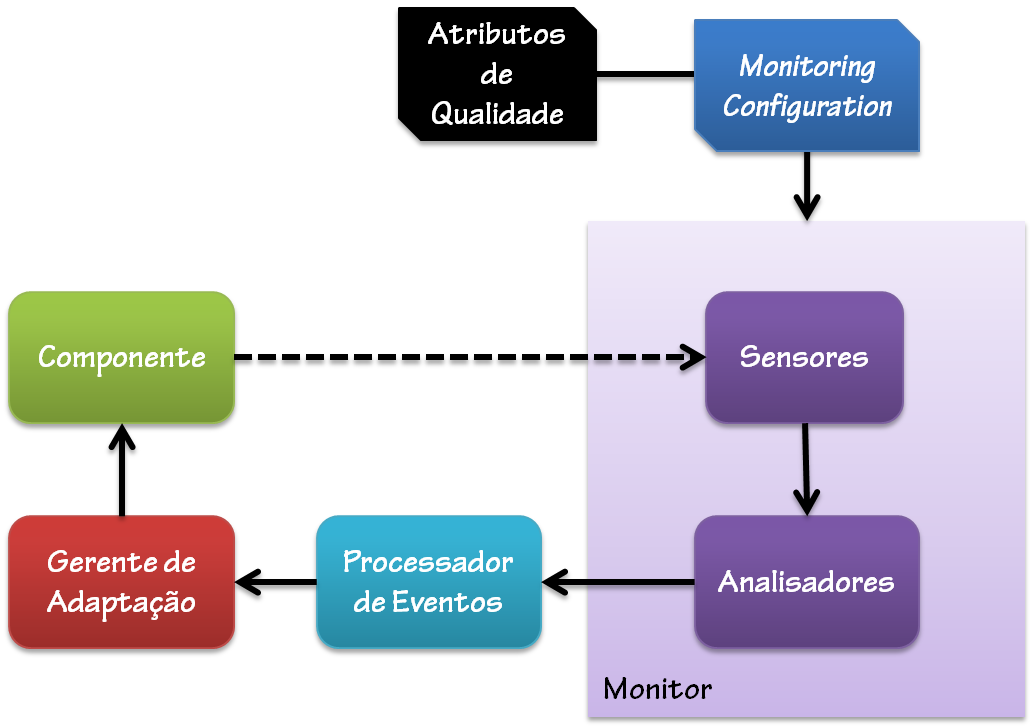
\includegraphics[width=11cm]{chapters/chapter3/monitor.png}
\caption{Sistema de Monitoração}
\label{fig:monitor}
\end{figure}


\section{Objetivo}
%TODO: objetivos DSOA

\section{Arquitetura}
\label{sec:dsoa_arch}

\begin{figure}[htp]
\centering
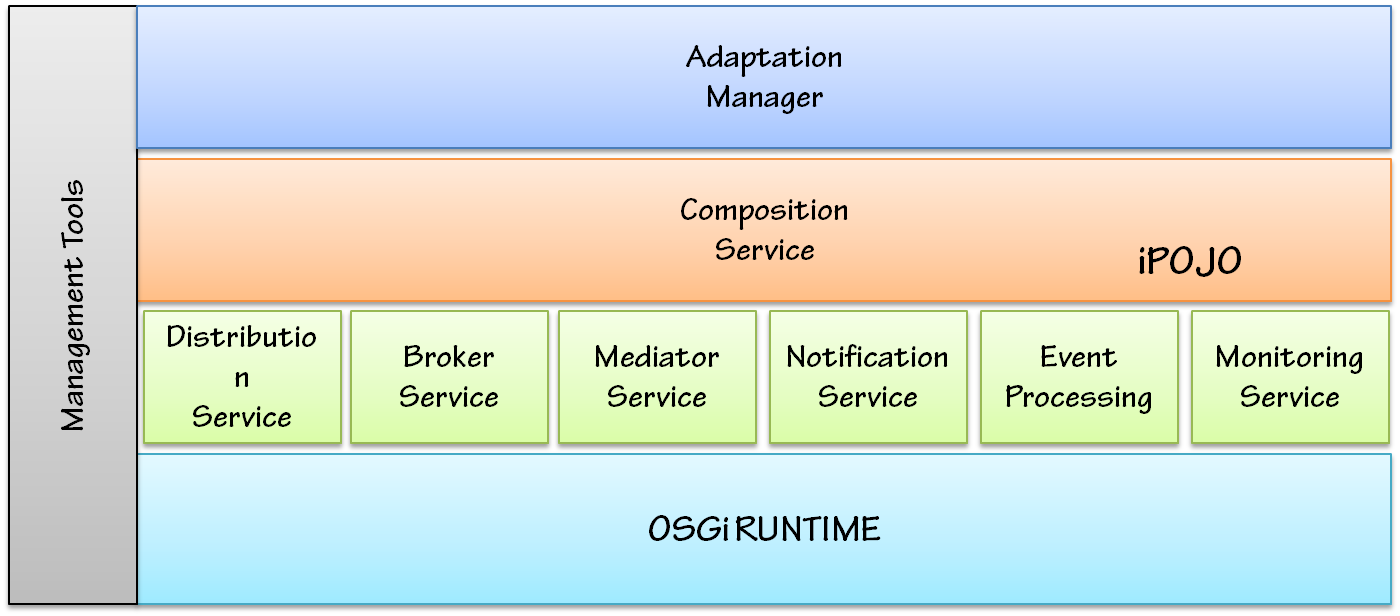
\includegraphics[width=13cm]{chapters/chapter3/dsoa-arch.png}
\caption[Arquitetura em Camdas DSOA]{Arquitetura em Camdas DSOA.}
\label{fig:proposal}
\end{figure}
%TODO arquitetura DSOA

\subsection{\textit{Distribution Service}}
%TODO

\subsection{\textit{Broker Service}}
%TODO

\subsection{\textit{Mediator Service}}
%TODO

\subsection{\textit{Notification Service}}
%TODO

\subsection{\textit{Event Processing Service}}
\label{subsec:cep}
%TODO

\subsection{\textit{Monitoring Service}}
\label{subsec:monit_serv}
%TODO

\subsection{\textit{Composition Service}}
%TODO

\subsection{\textit{Adaptation Manager}}
%TODO

\subsection{\textit{Management Tool}}
%TODO


\chapter{Solução Proposta}
\label{ch:4}

Neste capítulo, apresentaremos os componentes desenvolvidos para a realização dos objetivos propostos, bem como, detalhes de implementação considerados importantes para o melhor entendimento técnico do mecanismo. 

Também será mostrada uma análise do processo de gerenciamento automático, tendo em vista as ideias do ciclo PDCA, apresentado na Seção \ref{sec:pdca} deste trabalho. Essa análise irá relacionar as etapas definidas no ciclo com os sub-processos definidos pelo mecanismo.

\section{Visão Geral}
O contexto ao qual este trabalho está inserido, foi apresentado no capítulo \ref{ch:3}, através da plataforma DSOA, que provê um ambiente de composição dinâmica baseado em componentes orientados a serviços, com percepção de requisitos não-funcionais mapeados em atributos de qualidade. 

Porém, o estado atual da plataforma não dá suporte ao gerenciamento e monitoramento do provedor de serviços. O provedor basicamente define um conjunto de atributos de qualidade, que são utilizados pelos consumidores na seleção de serviço e na elaboração de contratos.

Atacar tais limitações mostra-se relevante, a medida que a qualidade do serviço é um fator chave tanto seleção do provedor quanto na manutenção dos contratos.

Buscando resolver esse problema, o objetivo deste trabalho é especificar e construir um mecanismo de gerenciamento automático de provedores de serviço, focado na prevenção de possíveis quebras de contrato. 

Para isso, a plataforma deve ser capaz de monitorar e adaptar dinamicamente o provedor de serviços, em função do contexto em que o mesmo executa.


\section{Arquitetura}
\label{sec:arch_prop}

Como vimos na Seção anterior, a plataforma DSOA, não prevê o gerenciamento do provedor de serviços com base em atributos de qualidade, deste modo, propomos uma extender a plataforma para suprir tais necessidades.

Para isso, foram desenvolvidos e implantados 2 módulos à plataforma. Um módulo de monitoração de recursos de hardware e um módulo de gerenciamento de provedores de serviços, ver Figura \ref{fig:proposal}.

O módulo de monitoração de recursos consiste em um sensor que captura informações referentes ao estado dos recursos da máquina. É instrumentado através de JMX e foi disponibilizado como um serviço da plataforma. 

O módulo de gerenciamento de provedor de serviço estende um \textit{container} fornecendo suporte a reconfiguração dinâmica de serviços. A reconfiguração é baseada em atributos de qualidade e no contexto em que o provedor executa.

A figura \ref{fig:proposal} destaca onde o trabalho desenvolvido esta situado na plataforma DSOA.

\begin{figure}[htp]
\centering
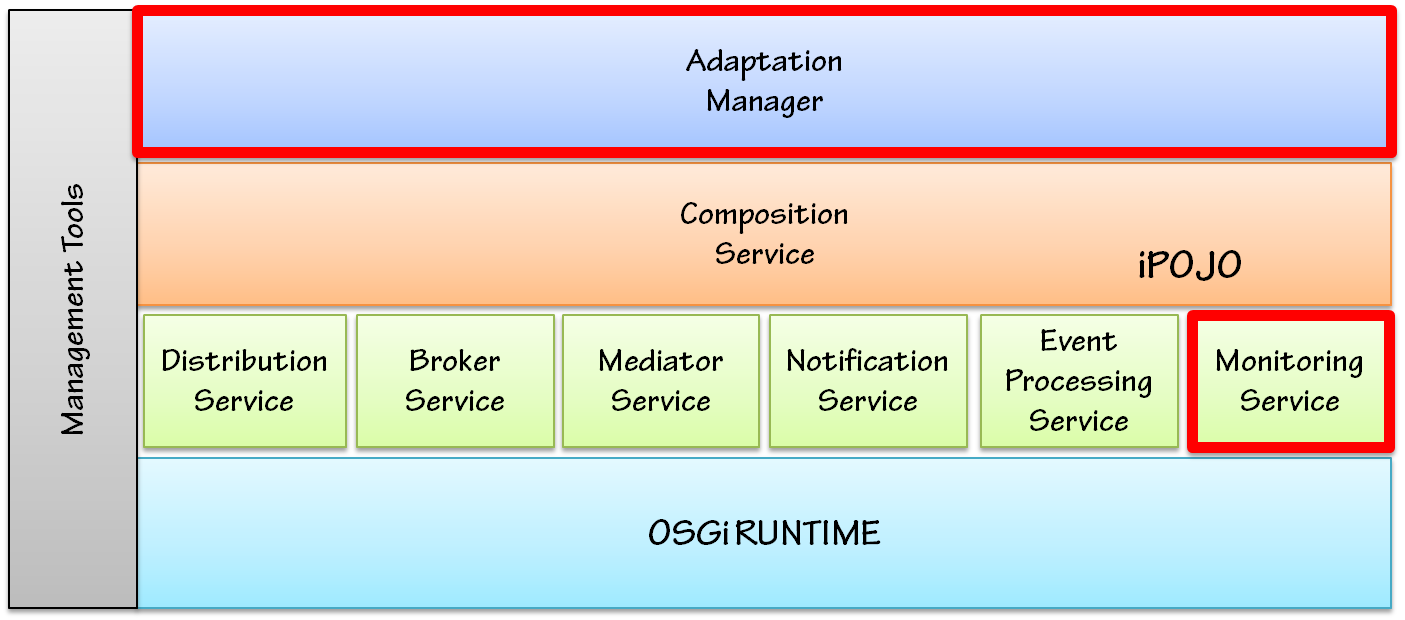
\includegraphics[width=13cm]{chapters/chapter4/dsoa-provider-manager.png}
\caption[Visão Geral da Proposta na Arquitetura]{Visão Geral da Proposta na Arquitetura.}
\label{fig:proposal}
\end{figure}

A combinação destes 2 módulos, junto aos serviços providos pela plataforma, surge como uma solução para o problema de gestão de provedores de serviço. Detalharemos seu funcionamento e arquitetura nas próximas seções.


\subsection{Módulo de Monitoração de Recursos}

Conforme o Capítulo \ref{ch:3}, um elemento importante de um sistema de monitoração corresponde a figura dos sensores. Sensores são responsáveis por coletar dados referentes aos recursos monitorados. E na plataforma DSOA, estão representados pelos serviços de monitoração. 

Originalmente a plataforma suporta um conjunto de sensores responsáveis pela coleta de dados referente a qualidade do serviço. Contudo, do ponto de vista do provedor, 2 fatores impactam diretamente na qualidade: a demanda e a limitação dos recursos de hardware e software~\cite{ye2011models}. 

Neste contexto, é vital que os recursos sejam monitorados, de forma a evitar que o consumo elevado degrade a qualidade do serviço provido, prevenindo eventuais quebras de contratos.

Essa necessidade nos levou a proposição de um novo conjunto de sensores, com a finalidade coletar dados relacionados ao contexto de execução do serviço, em termos de consumo de recursos de hardware, em particular, consumo de CPU e memória. 

Esse conjunto de sensores, foi incorporado à plataforma DSOA, através do serviço de monitoração de recursos (\textit{Resource Monitoring Service}), que é parte integrante do serviço de monitoração (\textit{Monitoring Service}), conforme a Figura \ref{fig:resc_module}.

\begin{figure}[htp]
\centering
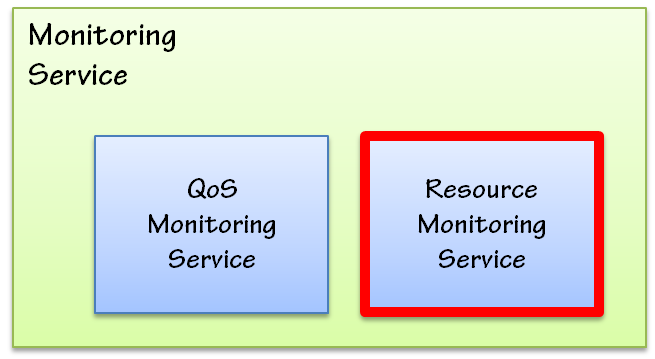
\includegraphics[width=9cm]{chapters/chapter4/monitoring-service.png}
\caption[Resource Monitoring Service]{Resource Monitoring Service.}
\label{fig:resc_module}
\end{figure}

Como foi dito na Seção \ref{sec:arch_prop}, o serviço de monitoração de recursos foi desenvolvido utilizando JMX para realizar a coleta de dados acerca dos recursos da máquina. Esse processo é realizado através de uma técnica de \textit{polling}~\cite{patterson2005organizacao} sobre os dados de mémoria e utilização de CPU.

Os dados do monitoramento são enviados, através da figura de eventos, ao serviço de processamento de eventos (\textit{Event Processing Service}), que gera notificações ao gerenciador de adaptação (\textit{Adaptaion Manager}) quando o provedor encontra-se em um ``Estado de Alerta''.

Um estado de alerta pode ser visto como uma iminência de quebra de contrato. Onde o provedor chegou a um ponto crítico de utilização dos recursos e logo não poderá garantir a qualidade devida, necessitando de adaptar-se ao novo contexto de execução.

\subsection{Módulo de Gerenciamento de Provedor}

Em linhas gerais, um processo de garantia de qualidade envolve um ciclo de atividades compreendendo além da coleta e análise dados, uma intervenção que representa uma ação ou conjunto de ações realizadas com base nessa análise. 

Na plataforma DSOA, as etapas de coleta e análise são tratadas respectivamente pelo serviço de monitoração e pelo serviço de processamento de eventos. A ação é de resposabilidade do gerente de adaptação, que no contexto do provedor de serviços, atualmente não realiza nenhum tipo de tratamento.

Deste modo, verificou-se a necessidade de estender o gerente de adaptação para atuar também no contexto do provedor, uma vez que, o monitoramento de recursos é restrito apenas à identificação de estados de alerta.

Assim, o módulo de gerenciamento do provedor (\textit{QoS Provider Manager}) implementa uma extensão do \textit{container} com o  objetivo de permitir que este se adapte dinamicamente, em função do estado atual de consumo de recursos e da qualidade do serviço provido. Essa extensão é apresentada na Figura \ref{fig:adapt_module}.


\begin{figure}[htp]
\centering
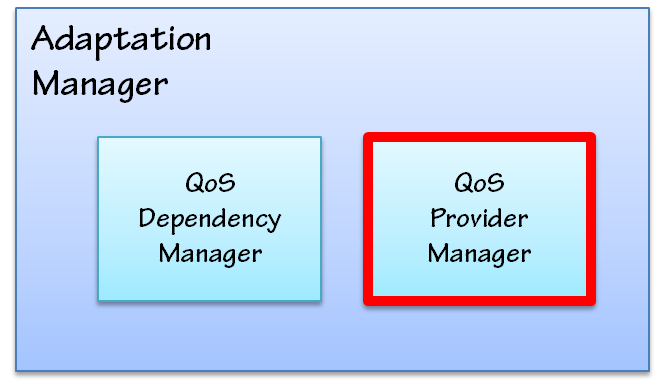
\includegraphics[width=9cm]{chapters/chapter4/adaptation-manager.png}
\caption[QoS Provider Manager]{QoS Provider Manager.}
\label{fig:adapt_module}
\end{figure}

O módulo de gerenciamento do provedor é capaz de adaptá-lo a seu contexto de execução, visando manter a qualidade de serviço, através do gerenciamento das políticas de criação de instâncias.

Em ~\cite{volter2005remoting}, temos um capítulo dedicado ao gerenciamento de ciclo de vida dos objetos remotos. Onde são apresentados diversos cenários de utilização ou limitação de recursos e o padrão de criação de instâncias que melhor se adapta a ele.

A partir disto, definimos um conjunto de políticas para cenários específicos de uso dos recursos. Porém, devido a diversidade enorme de cenários existentes, uma vez que, o uso de recursos é extremamente variável de aplicação para aplicação, a melhor maneira de contemplar a maioria dos casos é disponibilizar a política de criação de instâncias como um serviço. 

Deste modo, abrimos um leque à criação de diversas abordagens de gerenciamento de instâncias, a medida que, a política de criação de instâncias é independente do gerenciador de adaptação e é provida como um serviço.


\section{Aplicação do Ciclo PDCA}
Todo o processo de monitoramento e adaptação será baseado nas etapas definidas pelo ciclo PDCA.

Como vimos na Seção \ref{sec:pdca}, o ciclo foca em manter ou melhorar a qualidade de processos, com base nas informações referentes a sua execução.

\begin{figure}[htp]
\centering
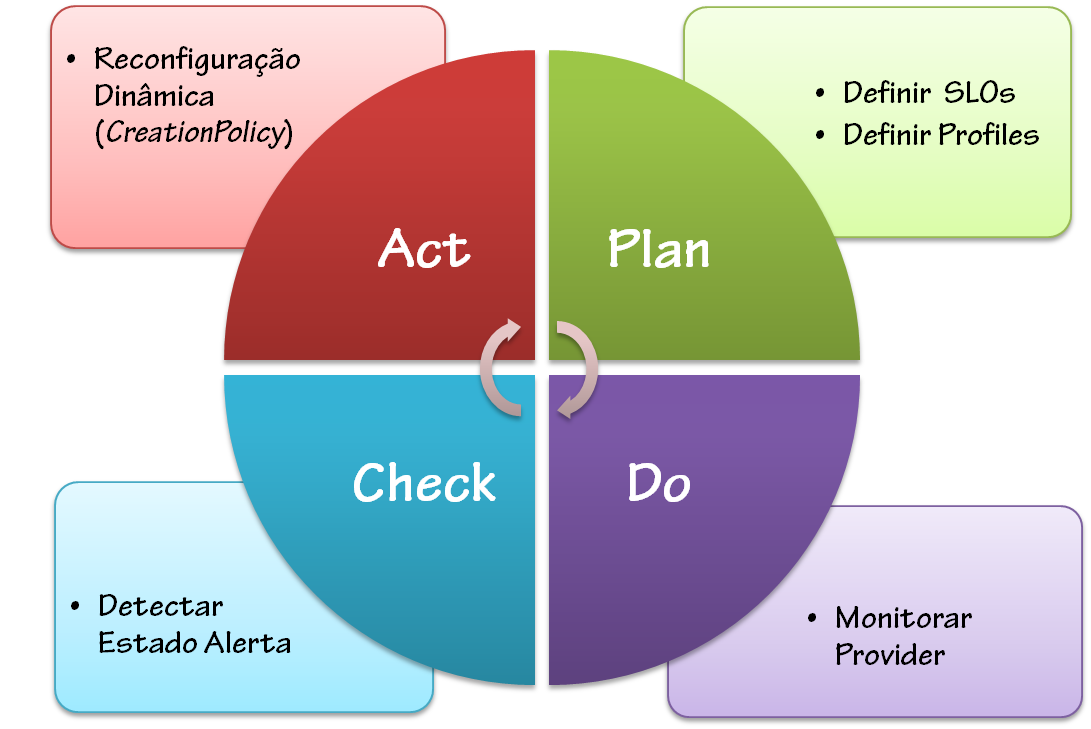
\includegraphics[width=10cm]{chapters/chapter4/pdca_actions.png}
\caption[Aplicação do Ciclo PDCA]{Aplicação do Ciclo PDCA.}
\label{fig:pdcamapping}
\end{figure}

\subsection{Plan}
Na etapa de planejamento, as metas serão definidas por meio de um documento XML~\cite{xml} que descreve as capacidades que o provedor afirma garantir. Essas propriedades são utilizadas para definir configurações de monitoração (\textit{Monitoring Configuration}), relacionadas a atributos de qualidade do provedor (\textit{e.g} tempo de processamento).

Essas metas são definidas através da \textit{tag} \verb slo , que descreve uma métrica a ser medida, um valor de \textit{threshold} e uma relação de limite(máximo ou mínimo) que o valor do \textit{threshold} pode ultrapassar. Em alguns casos, temos também o indentificador da operação provida. Essa informação é útil em casos de configurações de monitoração relacionadas a invocações de determinados métodos do provedor (e.g. \textit{throuhput} de uma operação). Ver Apêndice \ref{subsec:slo}.

Além disso, também são definidos no mesmo XML, métodos que visam atuar sobre estados de alerta, buscando garantir que as capacidades apresentadas sejam devidamente providas.

Esses métodos são descritos pela \textit{tag} \verb profile , que define um conjunto de \verb profiles ~responsáveis por relacionar as configurações de monitoração às políticas de gerenciamento de instâncias, onde cara política de gerenciamento tem por objetivo evitar a degradação da qualidade provida. 

Um \textit{profile} especificar um conjunto de \verb resources , semelhantes aos \textit{slos}, com o objetivos de definir uma configuração de monitoração


\begin{figure}[htp]
\centering
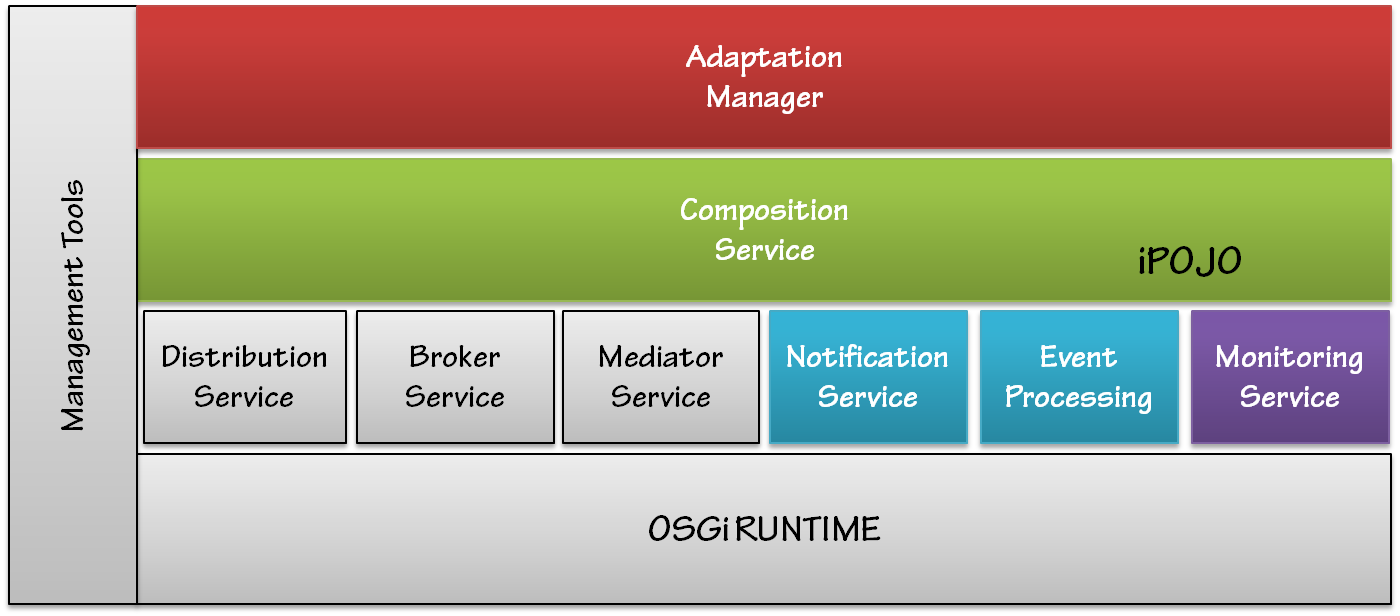
\includegraphics[width=13cm]{chapters/chapter4/pdca_arch_overview.png}
\caption[Componentes da Arquitetura x Fases PDCA]{Componentes da Arquitetura x Fases PDCA.}
\end{figure}


% Referencias
% Styles: http://amath.colorado.edu/documentation/LaTeX/reference/faq/bibstyles.html#styles
\bibliographystyle{unsrt}
\bibliography{references}
\addcontentsline{toc}{chapter}{Referencias Bibliográficas}


% Apendice
\clearpage
\addappheadtotoc
\appendix
\appendixpage
\chapter{JMX}

Este apêndice mostra exemplos de códigos JMX.\\

\section{Standard Mbean}

\subsection*{\!\textsl{\textbf{HelloMbean.java}}}
\begin{verbatimtab}[4]
package br.ufpe.cin.jmx.mbean;

public interface HelloMBean {
	public void setMessage(String msg);
	public String getMessage();
	public String sayBye();
}
\end{verbatimtab}

\subsection*{\!\textsl{\textbf{HelloMbean.java}}}
\begin{verbatimtab}[4]
package br.ufpe.cin.jmx.mbean;

public class Hello implements HelloMBean {

	private String msg;

	public Hello() {
		msg = "Hello World";
	}

	@Override
	public void setMessage(String msg) {
		this.msg = msg;

	}

	@Override
	public String getMessage() {
		return this.msg;
	}

	@Override
	public String sayBye() {
		return "bye";
	}
}
\end{verbatimtab}

\subsection*{\!\textsl{\textbf{Main.java}}}
\begin{verbatimtab}[4]
package br.ufpe.cin.jmx.mbean;

import java.lang.management.ManagementFactory;

import javax.management.MBeanServer;
import javax.management.ObjectName;

public class Main {

	public static void main(String[] args) throws Exception {

		MBeanServer server = ManagementFactory.
				getPlatformMBeanServer();
		ObjectName name = new ObjectName(
				"br.ufpe.cin.jmx.mbean:type=Hello");
		HelloMBean mbean = new Hello();

		server.registerMBean(mbean, name);
		Thread.sleep(Long.MAX_VALUE);
	}
}
\end{verbatimtab}


\end{document}
